\documentclass[format=sigplan, review=true]{acmart}

\usepackage{tikz}
\usetikzlibrary{shapes,arrows}
\usetikzlibrary{arrows.meta}

\newcommand{\hotspot}[0]{hot spot}
\newcommand{\hotspots}[0]{hot spots}
\newcommand{\coldspot}[0]{cold spot}
\newcommand{\coldspots}[0]{cold spots}
\newcommand{\hotspotcost}[0]{\textit{hotSpotCost}}
\newcommand{\unfit}[0]{unfit}
\newcommand{\dangerous}[0]{dangerous}
\newcommand{\useful}[0]{useful}
\newcommand{\useless}[0]{useless}
\newcommand{\Ao}[0]{\textsc{Autobahn 1.0}}
\newcommand{\At}[0]{\textsc{Autobahn 2.0}}
\newcommand{\fit}[0]{fit}
\newcommand{\preopt}[0]{pre-search}
\newcommand{\postopt}[0]{post-search}
\newcommand{\Preopt}[0]{Pre-search}
\newcommand{\Postopt}[0]{Post-search}
\newcommand{\absim}[0]{\textit{absenceImpact}}
\newcommand{\nonterm}[0]{non-terminating}
\newcommand{\unimp}[0]{unimproved}

\begin{document}
\acmJournal{PACMPL}
\title{Autobahn Minimizer}
\acmConference[Haskell'18]{11th ACM SIGPLAN International Haskell Symposium}{September 27-28, 2018}{St.Louis, MO, United States}
\author{Marilyn Sun}
\affiliation{Tufts University}
\email{marilyn.sun@tufts.edu}
\author{Kathleen Fisher}
\affiliation{Tufts University}
\email{kfisher@eecs.tufts.edu}
\begin{abstract}
	While lazy evaluation has many advantages, it can result in serious performance costs. Fortunately, Haskell allows users to enforce eager evaluation at certain program points by inserting bangs, which are strictness annotations. However, manual placement of bangs is both labor intensive and difficult to reason about. The Autobahn optimizer uses genetic algorithms to automatically infer bang patterns that improve runtime performance. However, Autobahn often generates very large numbers of bangs for each program. This is an issue for the user because each bang that cannot be deemed safe by the GHC compiler requires manual inspection to prevent the bang from introducing program non-termination.

This paper presents an improved version of Autobahn, which uses GHC profiling feedback to reduce the number of unnecessary bangs generated. \At{} adds a \preopt{} phase before the genetic algorithm to adjust the search space size, and a \postopt{} phase at the end to individually test and remove useless bangs. On average, the \preopt{} phase alone was able to eliminate 63 locations for potential bang placement per 100 LOC, and reduced the number of bangs eventually generated by 5 bangs per 100 LOC. Overall, \At{} reduced the number of bangs generated from 11 bangs to 1 bangs per 100 LOC, while only slowing program runtime by 3\%. Autobahn used in conjunction with these two phases allows users to obtain faster versions of their programs without the burden of manually checking through large numbers of bangs.
\end{abstract}
\maketitle

\section{Introduction}

\subsection{Lazy Evaluation}

Lazy evaluation is a property of Haskell that improves program efficiency and provides programmers the ability to use infinite data structures. Under lazy evaluation, expressions are only evaluated when their values are needed. Every unevaluated expression is stored in a \textit{thunk}, and its evaluation is delayed until another expression demands the value of the current one. Most of the time, this greatly improves program performance as it avoids wasting time on evaluating unnecessary expressions. It also means that users can operate on infinite data structures by only evaluating finite portions of it.

While lazy evaluation reaps many benefits, it can also create serious performance slow downs when too much memory is allocated to a large number of thunks. We can reduce the quantity of thunks by avoiding creating them for expressions that we know will eventually be evaluated. To avoid the creation of a thunk, programmers can insert strictness annotations such as bang patterns at certain program points to enforce eager evaluation. However, programmers need to distinguish program points that will benefit from eager evaluation from program points that do not need to be evaluated or will not terminate when evaluated. This task is difficult and often reserved for expert Haskell programmers. 

\subsection{Autobahn}

\textsc{Autobahn} is a Haskell optimizer that allows programmers to reduce thunks in their program by automatically inferring strictness annotations. Users provide \textsc{Autobahn} with an unoptimized program, representative input, and an optional configuration file to obtain an optimized version of the program over the course of a couple of hours. 

\textsc{Autobahn} uses a genetic algorithm to randomly search for beneficial locations to place bangs in the program. The genetic algorithm iteratively measures the performances of a series of candidate bang placements. Candidates that improve upon the original program's performance are preserved, and candidates that trigger non-termination or worsen program performance are eliminated. \textsc{Autobahn} eventually returns the user with a list of well-performing candidates, ranked by how much each candidate improves program performance. Users can then inspect the candidate bang placements, and decide if they want to apply one of them to the program.

\subsection{Too Many Bangs}

Candidates should be inspected before being applied because they can potentially introduce program non-termination when new input is given. Because \textsc{Autobahn} measures performance using representative input, the resulting candidate is optimized for that specific input. If a new type of input is supplied to the program after it is optimized, it could result in different behavior at program points that may cause the program to run forever. We can run GHC's static analysis after \textsc{Autobahn} to check for safe bangs, but it on average only marks 10\% of bangs as safe. This is because the analysis is necessarily conservative to guarantee termination on all inputs. 

In reality, bangs only need to be safe on inputs that the user will run it with. 
Because only the user will know the range of potential input types, only the user can inspect candidate bang placements and decide if they are safe to be applied. However, users face a time-consuming task of inspecting a large number of bangs when \textsc{Autobahn} generates too many bangs in a candidate. This occurs when the random genetic algorithm places many bangs throughout the program, including bangs that do not contribute much to program performance improvement. On average, \textsc{Autobahn} generates 11 bangs per 100 lines of code in its best performing candidates, and the user must manually inspect every one of those.   

\subsection{Autobahn 2.0}

This paper presents an improved version of \textsc{Autobahn} that aims to reduce the number of generated bangs. We refer to the original Autobahn optimizer as \Ao{}, and the improved version for bang minimization as \At{}. A \textit{\preopt{}} phase and \textit{\postopt{}} phase are each added before and after \Ao{} to locate and eliminate unnecessary bangs using GHC profiling. GHC profiles show the amount of runtime and memory each location in the program used. The \preopt{} phase adjusts the number of files that \Ao{} optimizes within a single program. \Ao{} is instructed to optimize files that contain locations that cost a large amount of resources, and to avoid optimizing files that do not contain costly locations. After \Ao{} runs, the \postopt{} phase individually tests each produced bang that falls within a costly location. Bangs that produce an insignificant impact on improving program performance are eliminated. On average, the addition of these two phases allows \At{} to produce 90.9\% fewer bangs than \Ao{}, while maintain similar runtime improvements. In this paper, I
\begin{itemize}
  \item demonstrate the effectiveness of the \preopt{} phase on programs from the NoFib benchmark suite that have had at least one file removed from consideration for optimization. There are 20 such programs in total. On average the \preopt{} phase reduced 63 potential bang locations per 100 LOC, and resulted in mean bang reductions of 63.38\%. 
  \item show that the \preopt{} phase's suggestions for additional files to optimize can improve \Ao{}'s optimization results by 86.6\% using the \textit{sumList} microbenchmark.
  \item POSTSEARCHDATA
  \item show that \At{} applied to the NoFib benchmark suite reduced the number of generated bangs from 11 bangs per 100 LOC to 1 bang per 100 LOC on average, while only increasing the optimized runtime by 3\%.
  \item use \At{} in a case study to optimize the performance of the \texttt{gcSimulator} garbage collector simulator. While the program runtime slowed down by 15\%, the number of bangs generated decreased by 81.9\%.
  \item apply \At{} in a second case study to show that it can preserve the application-specific annotations inferred by \Ao{} for the Aeson library. 
\end{itemize}


\section{Background}

\subsection{GHC Profiling and Cost Centres}
GHC provides a time and memory profiling system to allow users to better understand where their program spends 
the most time on. The
system adds annotations to the user's program and generates a report
detailing the amount of time, memory allocations or heap usage each 
location used. 

To generate these profiles, users simply run their program 
after re-compiling it with the profiling option and choose either a time and allocation or heap profile to generate, as well as the method in which the profiling 
system adds annotations. While users have the option to manually specify
annotations, \At{} uses the \texttt{-prof -fprof-auto} option, which
automatically adds an annotation around every binding that is not marked
INLINE in the program.

In the profile, these annotations are represented as cost centres with a 
certain cost associated with each of them. These costs indicate how much
time or memory resources each cost centre used as a percentage of the
whole program's resources. 

In order to minimize the number of bangs in 
a program while maintaining similar program performance, we need to 
preserve the bangs in the most costly cost centres and eliminate those 
located in the less costly cost centres. \At{} identifies a cost centre that consumes costs more than the \hotspotcost{} threshold as a \textit{\hotspot{}}. A cost centre that does not consume more than the \hotspotcost{} threshold is a \textit{\coldspot{}}. Currently, we set the \hotspotcost{} threshold to 6\% of the the overall program runtime, although that threshold can be
adjusted. As the threshold increases, fewer bangs
are preserved at the risk of a higher possibility of compromised program 
performance. 

\subsection{Genes and Chromosomes}

Cost centre profiling provides guidance for the otherwise random search 
that Autobahn performs using genetic algorithms. In the algorithm, any 
program source location where a bang may be added is represented as a \textit{gene} that can 
be turned on or off. A \textit{chromosome} is composed of all of the genes within a 
program and represented as a fixed-length bit vector, in which the bit value 
indicates the presence or absence of a bang. Since a program is a collection of source files, it is represented as a collection of bit vectors, or chromosomes.

\subsection{\Ao{}'s Genetic Algorithm}

\Ao{}'s genetic algorithm evaluates and manipulates randomly generated chromosomes. It repeatedly generates new chromosomes before measuring their performance using a fitness function. We call a chromosome that either significantly slows down program performance or causes non termination an \textit{\unfit{}} chromosome. If the fitness function determines that a chromosome is \unfit{}, the chromosome is immediately discarded. If the fitness function determines that a chromosome behaved well, the chromosome is deemed \textit{\fit{}} and kept for future rounds of generation. 

For each round of chromosome generation, \Ao{} introduces randomness by performing either a mutation or a crossover. A mutation flips a gene in the chromosome whenever a randomly chosen floating point number exceeds the \textit{mutateProb} threshold. A crossover combines two chromosomes by randomly picking half of the genes from each parent chromosome. For either of these random operations, \Ao{} uses a unique number generator each time to guarantee randomness. 

\subsection{Representative Input}

To run \Ao{}, users need to provide representative input to their program. The input should be short enough for \Ao{} to finish execution in a reasonable amount of time while still be long enough for it to measure noticeable time improvements if there are any. Ideally, representative input should also be as similar to the typical use case of the program as possible to reduce chances of unexpected behavior after optimization when using different types of program input.

Similarly, the quality of representative input impacts the quality of \At{}'s performance as well, because different types of input may generate wildly different results in GHC profiles. Therefore, the user must carefully choose their program's representative input.

\section{\At{}}
\subsection{Why Too Many Bangs Are Generated}

The first step to eliminating bangs is to identify categories of bangs and hypothesize the reason why each category exists. A \textit{\dangerous{}} bang is a bang that can significantly slow down program runtime or cause program non-termination. A \textit{\useful{}} bang improves program performance, and a \textit{\useless{}} bang neither improves nor worsens program performance. 

While an \unfit{} chromosome may perform poorly as a whole, it can contain a mixture of \dangerous, \useful{} and \useless{} bangs. \Ao{} handles \unfit{} chromosomes by discarding them entirely, but fails to provide a method of isolating the specific \dangerous{} bangs in an \unfit{} chromosome. It is necessary to isolate and remove \dangerous{} bangs because they might otherwise reappear in later generations as a result of random mutation. 

Fit chromosomes also face a similar issue. \Ao{} handles \fit{} chromosomes by preserving the entire chromosome, without separately identifying the \useful{} bangs from the \useless{} ones. This is problematic for two reasons. Firstly, we might lose \useful{} bangs in future rounds of generations because we cannot track them and guarantee that random methods of mutation and crossover will preserve them. Secondly, \useless{} bangs could survive by being grouped with \useful{} bangs even though they should be eliminated. The accumulation of such bangs can dramatically increase the number of bangs in a program, leaving it up to the user to identify potentially unsafe bangs from the safe ones. 

We hypothesize that \Ao{} generates copious amounts of bangs because it is incapable of identifying categories of bangs within the same chromosome. The further addition of randomness means that the entire chromosome is repeatedly searched as the search space is never definitively reduced. Because there is a fixed number of genes in a program, the search space for the genetic algorithm is also equivalently fixed. Therefore, as the program source code increases in size, the algorithm also generates significantly more bangs as chromosomes increase in size. 

\subsection{The Solution}

\At{} uses GHC profiling to do what Autobahn cannot: isolate portions of a chromosome by their individual contributions to program performance. Cost centres not only break down a chromosome into smaller portions by source code bindings, but their associated costs also imply how likely a bang placement will affect program performance. If executing code at a \hotspot{} occupied a significant portion of the overall program runtime, then a bang-induced change in performance at the \hotspot{} will likely significantly affect overall runtime as well. 

There are two ways to apply GHC profiling information to reduce the number of generated bangs. The first way is by reducing the previously fixed size of the initial chromosome. Because \Ao{}'s search space is directly correlated to the size of the program source code, we can reduce the search space by eliminating all files that only contain \coldspots{} prior to Autobahn's optimization. Since \useless{} bangs are most likely later generated and located within \coldspots{}, early elimination of genes in \coldspots{} is beneficial. 

However, \hotspots{} can contain a mixture of \useful{} and \useless{} bangs as well. To definitively eliminate \useless{} bangs and preserve \useful{} bangs, we can individually isolate and measure the performance of each bang in each \hotspot{}. The effects of combining bangs is hard to predict, but the permutation size of all possible combinations of the remaining bangs can grow very large. To simplify the process, we adopt the method of individually turning off one bang at a time to test. We can then exhaustively test each bang because the number of \hotspots{} in a program is limited. This testing process relies on \Ao{}'s randomly generated winning combination of bangs as a starting point. Both of these methods are later explained in full detail, and a diagram of the workflow is shown below.
\newline
\tikzset{%
  >={Latex[width=2mm,length=2mm]},
            base/.style = {rectangle, rounded corners, draw=black,
                           minimum width=4cm, minimum height=1cm,
                           text centered, font=\sffamily},
  activityStarts/.style = {base, fill=blue!30},
       startstop/.style = {base, text width=4cm, fill=red!30},
    activityRuns/.style = {base, fill=green!30},
         process/.style = {base, text width=3cm, fill=orange!15,
                           font=\ttfamily},
}

\begin{tikzpicture}[node distance=1.5cm,
    every node/.style={fill=white, font=\sffamily}, align=center]
  \node (preo)             [activityStarts]              {\Preopt{}};
  \node (user)     [process, left of=preo, xshift=-3cm]          {Original Program, Representative Input, Autobahn Configuration};
  \node (autobahn)      [activityStarts, below of=preo, yshift=-2.5cm]
                                                      {\Ao{}};
  \node (end)      [startstop, left of=autobahn, xshift=-3cm, yshift=1cm]
                                                       {If program is unsuitable for optimization: Alert user and end process};
                                                  
  \node (posto) [activityStarts, below of=autobahn, yshift=-2cm]
                                                    {\Postopt{}};     
  \node (endmin)      [startstop, below of=end, yshift=-1cm]
                                                       {If negligible optimization improvement: Alert user and end process};                                                       
   \node (result)     [process, left of=posto, xshift=-3cm, yshift=-1.5cm]          {Optimized and minimized program};                                                   

  \draw[->]             (preo) -- node[text width=4cm]
  					{Remove \coldspots{}, suggest external libraries, check if program is unsuitable for optimization}(autobahn);
  \draw[->]     (user) -- (preo);
  \draw[->]      (autobahn) -- node[text width=4cm]
  					{Find winning chromosome using genetic algorithms}(posto);
   \draw[->]      (preo) -- (end);
   \draw[->]      (posto) -- (endmin);
  \draw[->]      (posto) -- node[text width=4cm, xshift=-2cm, yshift=0.8cm] {Individually test each bang in winning chromosome}
                                   (result);
  \end{tikzpicture}


\subsection{Autobahn Coverage}

By default, Autobahn optimizes all files in the program directory. Users can specify optimization coverage by manually adding or removing file paths while configuring Autobahn. Although Autobahn does not consider external libraries imported in the source code, users can manually add local copies of external libraries in the program directory for optimization. 

However, just as manually reasoning about the placement of bangs is difficult, users generally find it difficult to reason about which files should or should not be optimized. By examining GHC profiles, we can have a much better idea of which files to eliminate based on whether or not they contain \hotspots{}. Combining this knowledge with the option to configure Autobahn coverage, we can now manipulate the initial chromosome size by units of file sizes. 

\subsection{\Preopt{} Profiling}

\Preopt{} profiling does more than just reducing existing search space. Instead, it guides, redirects and expands the current search space to maximize efficiency and performance prior to \Ao{}'s optimization. Because chromosome sizes directly influence the number of generated bangs, search space manipulation can minimize the possibility of generating \useless{} or \dangerous{} bangs and maximize the chances of generating \useful{} ones.

To reduce the initial search space, the \preopt{} phase begins by generating a GHC time and allocation profile for the unoptimized program with user provided representative input. Then, the files that contain at least one \hotspot{} are identified. Files that do not contain \hotspots{} are eliminated from the Autobahn coverage of files. \Ao{} then optimizes the program as usual, except using a much smaller set of files and thus chromosomes to begin its genetic algorithmic search. 

There are three important impacts that \preopt{} profiling creates. First of all, it greatly reduces the number of bangs Autobahn generates by reducing the initial search space. Secondly, it identifies programs that are potentially unsuitable for Autobahn optimization. If a program contains a large set of cost centres that all contribute minimally to program runtime, there may not exist a single location in which placing a bang will make a significant difference in program runtime. If the \preopt{} identifies a program that only contains \coldspots{}, it will alert the user and save them the time and effort of running Autobahn when they will most likely see minimal performance improvements. Lastly, if a \hotspot{} is located in an external library file, the \preopt{} phase can suggest users which external libraries to add to the Autobahn coverage for better optimization results.

It is worth noting that although \preopt{} can reduce search space, it cannot reduce \Ao{}'s runtime as a result. Unless the search space is small enough to be exhaustively searched, \Ao{} will continue to search through it until the allotted runtime is up. So if a user allowed \Ao{} to run for four hours, it will continue to run for four hours regardless of search space size. However, reduced space allows \Ao{} to search more thoroughly and potentially find better results that it did not have time to find before. 

\subsection{\Postopt{} Bang Elimination}

After \Ao{} optimizes the search space and determines a winning chromosome, \At{} once again uses GHC profiling information to reduce the number of bangs in the winning chromosome. It begins by mapping each gene in the winning bit vector to their corresponding set of cost centres. 

For each gene in the bit vector, the \postopt{} phase filters out all of those that are already turned off and keep them turned off. It then examines genes that are turned on and fall within a \coldspot{}, and turns them off before filtering them out as well. We can turn them off because those genes are most likely \useless{} bangs. 

The remaining genes are the interesting ones that both contain a bang and fall within a \hotspot{}. These genes require further testing because even though \hotspots{} are likely to significantly reduce overall runtime when their own runtimes are reduced, we are unsure if the cost centre runtime was reduced in the first place. That is, placing a bang in a cost centre may not always improve performance at the cost centre. Therefore, genes within \hotspots{} that cannot be improved through the placement of bangs are also \useless{} and should be discarded.

\subsection{Testing \hotspots{}}
 
There are usually so few remaining genes that are both turned on and within a \hotspot{} that it is possible to exhaustively test them. The \postopt{} phase tests them by isolating and turning off each bang while keeping all other remaining bangs on. It then measures program runtime and compares it to the program performance of the winning chromosome determined by Autobahn. 

If the absence of this bang slows down the program by the \absim{} threshold, this bang is useful and kept in the pool of remaining bangs. If the bang's absence does not slow down the program by at least the \absim{} threshold, the bang is deemed \useless{} and discarded. The \absim{} threshold is adjustable and currently set to 5\%. The \postopt{} phase repeats this process for every bang to be tested, and the minimization result is the combination of surviving bangs by the end of testing.

\section{Implementation}

\subsection{Program Architecture}

The addition of \preopt{} search space reduction and \postopt{} bang reduction alters the original program architecture of \Ao{}. Prior to optimization, the original program is first profiled and evaluated for search space manipulation in the \preopt{} phase. \Preopt{} builds the user's program with profiling enabled, and runs the unoptimized version with the user provided representative input to obtain a time and allocation profile. The profile is only generated once, and the rest of of \At{} refers to the same profile throughout the entire program. Depending on the location of \hotspots{} indicated by the profile, the program's optimization coverage will either be automatically reduced or manually expanded by the user. 

Then \Ao{} is uses the same genetic algorithm to find a winning chromosome. It uses the \textit{haskell-src-exts} parser to parse source files and identify genes, then applies a genetic algorithm with a fitness function to search for the best performing chromosome.

The resulting chromosome is further tested and reduced using GHC profiling information in the \postopt{} bang reduction phase. After an initial pass of elimination to get rid of all turned-off bangs and bangs located in \coldspots{}, we individually test the impact of the absence of a turned-on bang in each \hotspot{}. If a bang meets the \absim{} threshold, it is kept in future rounds of testing and will remain in the final combination of bangs for the optimized program. If a bang does not meet the \absim{} threshold, it is removed for future rounds of testing and will not appear in the final combination. 

Bangs in \hotspots{} are tested in order of decreasing costs. While we recognize that the order in which we test them may affect their performance, it is simply too time consuming to test every possible combination of bangs in every possible order. For simplicity, we chose to only consistently test each individual bang once in order of decreasing costs. 

Finally, the \postopt{} phase returns the final combination of bangs that have survived each round of testing. If \Ao{} failed to find a chromosome that improved program runtime by 6\% to begin with, then the \postopt{} phase will refuse to minimize because the insignificant performance improvement indicates that users are better off keeping the original unoptimized program instead.


\subsection{Running \At{}}

A user runs \At{} the same way as they would run the \Ao{}. The user provides a copy of their program source code, representative input, and an optional Autobahn configuration file. Because both search space reduction and minimization after Autobahn typically do not require a significant amount of time, the user should barely notice an increase in the amount of time needed for optimization. 

If \At{} successfully ran, the user can find the minimized source code in the same project directory along with the usual Autobahn survivor and results directories. If \preopt{} profiling detected that the program is unsuitable for optimization, or if \Ao{} failed to significantly optimize the program, then \At{} would warn the user and halt the optimization process. If external libraries could be added to Autobahn's coverage to potentially boost optimization performance, the \preopt{} phase would alert the user and continue to optimize as normal.

\subsection{Source Locations}

Because each bit in a bit vector represents a gene in a chromosome, we modified the bit vector to indicate which cost centre each bit was located in as well. 
Cost centres are uniquely identified by source location in source files. We mapped each bit to its corresponding source line. To turn the bangs in a \hotspot{} on or off, we can traverse the bit-location vector and manipulate the bits that are tagged with source lines that fall within the range of that \hotspot{}'s source location.

\subsection{Removing Illegal Genes}

Unfortunately, the \textit{haskell-src-exts} parser that \Ao{} uses incorrectly identifies the left hand side of bindings within instance declarations as potential locations to place bangs. For that reason, files that contain instance declarations have been previously avoided and left unoptimized when testing \Ao{}. We wanted to support the optimization of these files in \At{}, so we removed any randomly generated illegal bangs prior to each round of fitness evaluation in the genetic algorithm. The rest of the genetic search and \At{} runs identically as before.

To keep track of whether a bang is legal, we used a validity-indicating boolean vector to represent whether each gene in the source code is legal. Prior to inserting bangs into a program, \At{} would check the validity of a gene against the boolean vector to make sure that the bang is located in a legal location.

Generically traversing the parser-generated AST using boilerplate code fails to identify illegal genes, so we needed to manually traverse it to construct the validity vector. As we traversed the tree, we kept track of whether a left hand side binding is within an instance declaration. If so, then that binding is an illegal bang location and is marked as a false boolean value in the validity vector. All other legal bang locations are marked as a true value.

\At{} successfully uses this method to avoid inserting bangs into illegal locations after being misguided by the parser. As a result, it allows us to optimize files that include instance declarations, which we previously avoided altogether when using \Ao{}. 

\section{Evaluation}

\subsection{Experiment Setup}

All versions of Autobahn were compiled using GHC version \texttt{8.0.2}. The NoFib benchmarks were also compiled with GHC version \texttt{8.0.2}, \texttt{-XBangPatterns} and enabled profiling along with NoFib's default flags. Our research did not test the certain benchmarks in the NoFib suite that failed to compile and run on their own and benchmarks that \Ao{} refuses to minimize because they already had very fast runtimes. There were 61 total remaining benchmarks that we ran experiments on.

In the runtime graphs for all sections below, a runtime value of 2.0 indicates that the optimized version of the program is \textit{\nonterm{}}. A runtime value of 1.0 indicates that the optimized version of the program had an identical runtime compared to the original version and is \textit{\unimp{}}.


\subsection{\Preopt{} Search Space Reduction}
To test how much search space can be reduced by the \preopt{} phase of \At{}, we ran \Ao{} with \preopt{} profiling on the NoFib benchmark suite. To account for fluctuation, we took the mean of running the program ten times on the benchmark suite. All runs were optimized on runtime only, and the \hotspotcost{} and \absim{} thresholds were both set to 6\%. 

Out of the 60 benchmarks, only 20 benchmarks had at least one file that was eliminated during the \preopt{} phase. The other 40 benchmarks either only had one file in the program to begin with or had zero files eliminated in the \preopt{} phase. These benchmarks would be optimized identically as running only \Ao{} would, so their results are not represented in a graph below. The 40 benchmarks also includes benchmarks that had zero files remaining after the \preopt{} phase and were marked as unsuitable for optimization. Those benchmarks are discussed in detail in Section 5.3.

Figure 1 includes results from the 20 benchmarks that had at least one file that was eliminated during the \preopt{} phase. The number of eliminated genes shows the number of potential bang locations that were eliminated before \Ao{} ran. Because most benchmarks do not have bangs in the original versions of their programs, the number of original bangs in Figure 1 is usually 0. Not every benchmark succeeded every time it was being optimized, and the failure run column indicates how often the benchmark was left unoptimized using \preopt{} and \Ao{}.

The \texttt{anna, expert,} and \texttt{symalg} benchmarks are particularly interesting because \Ao{} consistently failed to find winning chromosomes for them, so no bangs were generated. However, after reducing the search space using \preopt{}, \Ao{} was able to more thoroughly search a smaller and more focused space to find meaningful bangs. Therefore, \Ao{} was able to discover a set of performance-impacting bangs with the help of the \preopt{} phase. 

Figure 2 shows the corresponding runtime performance of results generated by \Ao{} and \Ao{} with the \preopt{} phase. The graph shows that even when a large number of genes are eliminated prior to optimization, the optimizer is still able to find \useful{} bangs that result in similar runtime improvement. This confirms that the eliminated genes were truly insignificant bang locations that are not worth spending time searching through. 

\begin{figure*}
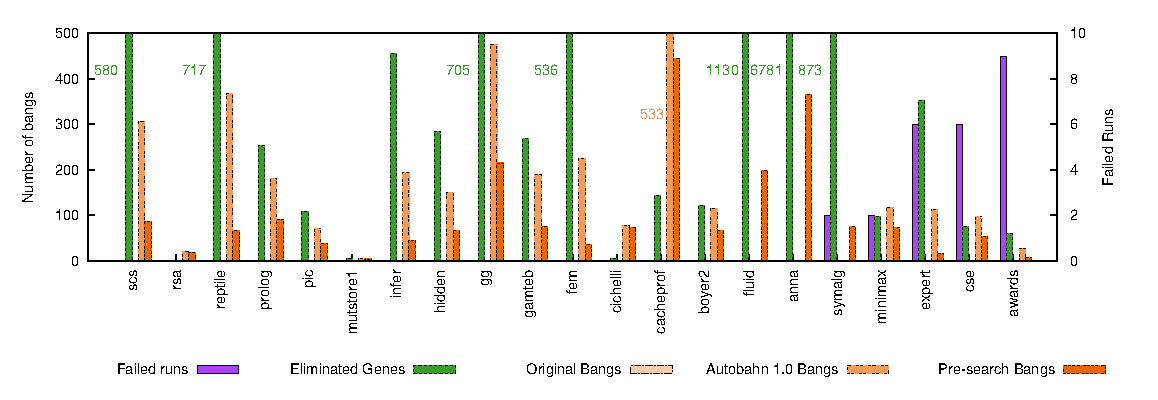
\includegraphics[width=\textwidth]{pre-aut-bangs}
\caption{Number of bangs generated by \Ao{} vs. \preopt{} phase combined with \Ao{} compared across 20 benchmarks. Columns that exceed the maximum axis value are labelled with their actual values.}
\end{figure*}

\begin{figure*}
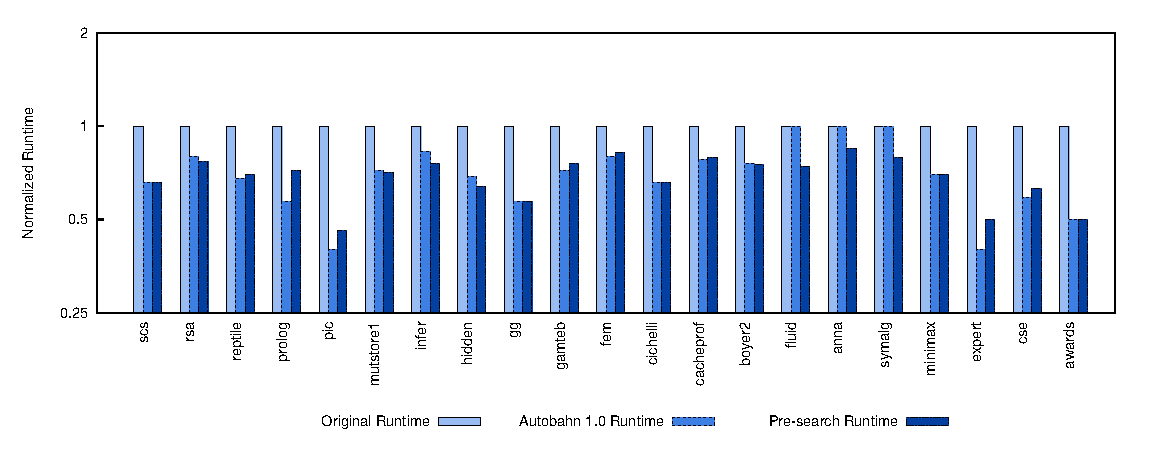
\includegraphics[width=\textwidth]{pre-aut}
\caption{Normalized runtime of \Ao{} results vs. \preopt{} phase combined with \Ao{} results across 20 benchmarks. The x-axis normalized runtime is on a log scale of base 2. Columns that exceed the maximum axis value are labelled with their actual values.}
\end{figure*}

\subsection{\Preopt{} File Elimination}

We have found six benchmarks in the NoFib suite that the \preopt{} phase identifies as unsuitable for optimization when the \hotspotcost{} threshold is set to 6\%. These are \texttt{awards, callback001, callback002, mutstore2, sorting,} and \texttt{threads007}. As expected, when attempting to optimize \texttt{awards}, \texttt{sorting} and \texttt{threads007}, \Ao{} consistently fails to optimize and returns the \unimp{} runtime code. However, Autobahn was able to successfully optimize the other programs. Through inspection, we concluded that \texttt{callback002} would've benefited from a lower \hotspotcost{} threshold as its most costly hot spot takes up 3.9\% of the program runtime. Both \texttt{callback001} and \texttt{threads007} would've benefited from inspecting heap profiles instead of time and allocation profiles as the costs associated with their hot spots were noticeably larger in heap allocations while remaining insignificant in runtime costs. The \texttt{mutstore2} program's performance fluctuated wildly even without bangs in it. For example, its measured runtime was as low as 60\% - 80\% of its original runtime in one third of the experiments we ran with no bangs in the program. Therefore, the optimization results were likely skewed by the fluctuating runtime.

\subsection{\Preopt{} File Addition}

To demonstrate the effectiveness of using the \preopt{} phase to expand Autobahn's coverage for improved optimization results, we tested our approach on the \texttt{sumList} microbenchmark. We created \texttt{sumList} to simulate the scenario in which a programmer references code from an external library or external file that contains \hotspots{} but is not within their current coverage range. 


The \texttt{sumList} program's \texttt{Main.hs} file contains only one function: a main function that constructs a list of integers from 1 to 1,000,000, and calculates the sum of all integers in the list using an external \textit{sum} function located in \texttt{Sum.hs}. The user may decide to set the optimization coverage to [\texttt{Main.hs}], because they are interested in making the main program run faster. However, as demonstrated in table 1, \Ao{} was only able to improve program performance by 3\%, even when it was able to exhaustively search the only six lines of code in the main function. Upon inspecting the results, the user may be mistaken in believing that their program runtime cannot be possibly improved further. 

But there are indeed other opportunities to speed up \textit{sumList} located in places that the user did not think about. The user decides to rerun the \Ao{} using the \preopt{} phase as well. GHC's time and allocation profile indicates that the largest \hotspotcost{} was 9.5\% and located in lines 7 to 8 in the \textit{sum} function in \texttt{Sum.hs}. The \textit{sum} function is entirely lazy and did not immediately compute the sum of each integer as it recursed through the list. In the resulting log file, the user is alerted about this fact through a message that advises them to consider adding \texttt{Sum.hs} to the list of files that \Ao{} optimizes. After expanding the coverage and running optimization again, \texttt{sumList} was able to run at only 13\% of the original runtime, a dramatic improvement compared to optimizing using \Ao{} alone.

Although the \texttt{sumList} example is short and simple, it shows the larger potential for users to obtain much better optimization results when running the \preopt{} phase in conjunction with \Ao{}. Programmers often build upon each other's code and use external functions that they may not be entirely familiar with or did not consider optimizing. The \preopt{} phase identifies valuable missed opportunities and improves \Ao{}'s optimization results. Of course, the addition of more files to optimize means that more bangs might be generated. It is up to the user to decide if they want to add the suggested files for better optimization results at the risk of them needing to inspect more bangs.
\newline
%We also ran experiments using the Aeson parser library that handles JSON files using either the \texttt{validate} or \texttt{convert} driver programs. \texttt{validate} simply checks if the file is written in valid JSON syntax, and \texttt{convert} actually converts file input into a Haskell data structure. 

%While running the \preopt{} phase on the Aeson library, we were suggested by the program to include files from the external \texttt{Data/Aeson} library in the Autobahn optimization coverage because the \texttt{Data/Aeson/InternalTypes.hs} file included multiple \hotspots{}. However, \texttt{InternalTypes.hs} already included manually inserted bangs by its author. Therefore we ran experiments using a version of \texttt{InternalTypes.hs} with no bangs in it to see if we could recreate the manually inserted bangs. If so, library authors could run Autobahn to place bangs in their files instead of manually doing so. 


\begin{tabular}{p{2.5cm}p{1.5cm}p{2cm}p{1cm}}
\hline
Version   & Coverage & Normalized Runtime & No.Bangs \\
\hline
Original      & N/A   &   1	 & 0   \\
\Ao{}       & [\texttt{Main.hs}]      & 0.97    &  2\\
Pre-optimization	& [\texttt{Main.hs}, \texttt{Sum.hs}]         & 0.13      & 4\\
\hline
\end{tabular}

%\begin{tabular}{llr}
%\hline
%Version   & Driver & Normalized Runtime \\
%\hline
%Original      & value   & 1     \\
%          & json        & 1      \\
%Pre-optimization       & value     & 0.73     \\
%          & json        & 0.66	\\
%\Ao{}       & value     & 0.56      \\
%          & json        & 0.72	\\
%\hline
%\end{tabular}

\subsection{\Postopt{} Bang Reduction}

To test the efficiency of reducing bangs using the \postopt{} phase, we compared the results of running only \Ao{} with \Ao{} and the \postopt{} phase. Similarly, we took the mean of running the program ten times on the NoFib benchmark suite while optimizing on runtime only, and set both \hotspotcost{} and \absim{} thresholds to 6\%. 


A benchmark is successfully optimized if \Ao{} improved its performance by at least 6\% after optimization. Figure 3 and Figure 4 include results from the 22 benchmarks that were consistently successfully optimized by \Ao{} in each run. [\textit{TODO insert inconsistently successful benchmarks results here}]

Figure 3 shows that the number of bangs eliminated by the \postopt{} phase is quite significant. Figure 4 shows the corresponding runtime performance of each optimized program. In most benchmarks, the \postopt{} phase does a little worse than running only \Ao{}, because the \absim{} threshold limits the remaining bangs to those that affect program runtime by at least 6\%. If a user wants to maintain more similar runtime results, they can lower the \absim{} threshold so the minimizer becomes less aggressive in bang elimination. That way, more bangs will be preserved, but runtime performance will improve. 

The interesting results for programs \texttt{anna} and \texttt{fluid} show that while \Ao{} found bangs that triggered a \nonterm{} runtime code, \postopt{} bang elimination was able to get rid of the \dangerous{} bangs that caused non termination. 

\begin{figure*}
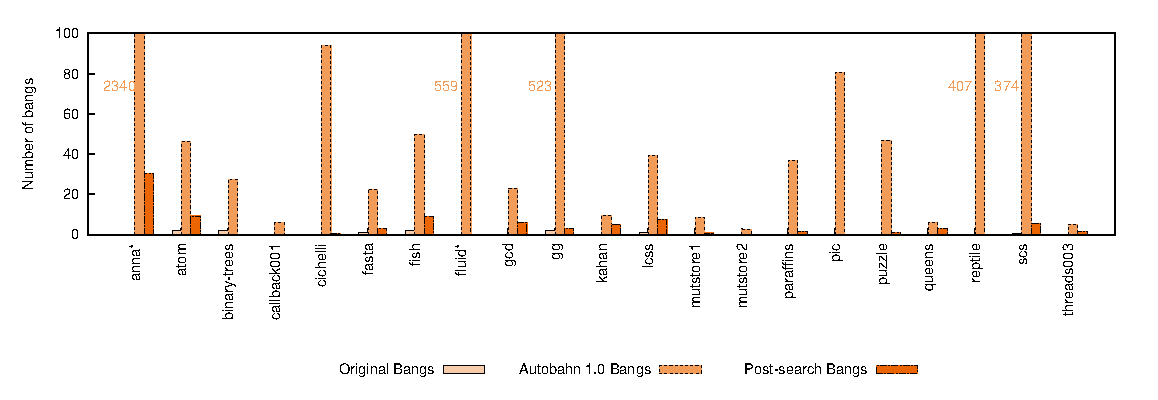
\includegraphics[width=\textwidth]{aut-post-bangs}
\caption{Number of bangs generated by \Ao{} vs. \postopt{} phase combined with \Ao{} across 22 benchmarks. Columns that exceed the maximum axis value are labelled with their actual values.}
\end{figure*}

\begin{figure*}
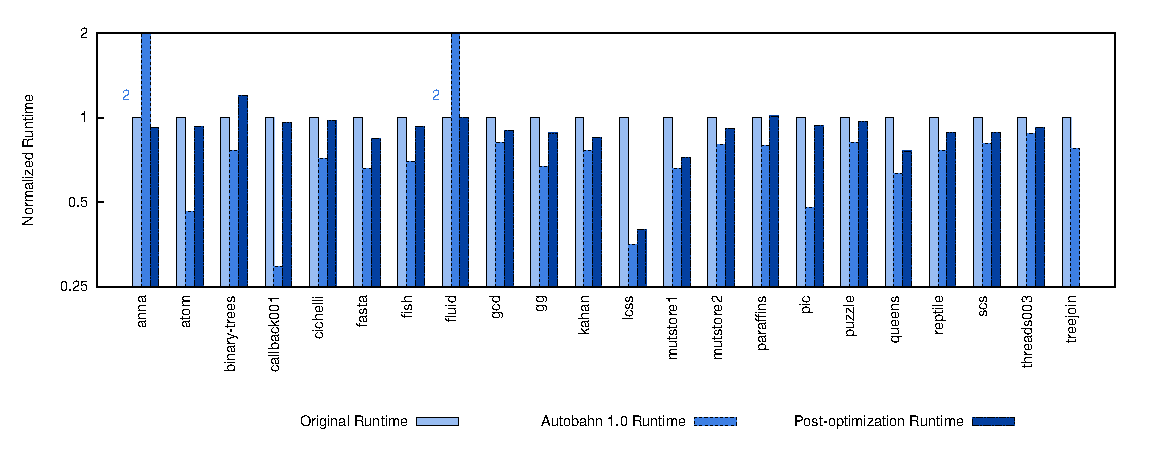
\includegraphics[width=\textwidth]{aut-post}
\caption{Normalized runtime of \Ao{} results vs. \postopt{} phase combined with \Ao{} results across 22 benchmarks. The x-axis normalized runtime is on a log scale of base 2. Columns that exceed the maximum axis value are labelled with their actual values. Benchmarks that did not terminate are indicated with a 2.0 \nonterm{} code runtime.}
\end{figure*}

\begin{figure*}
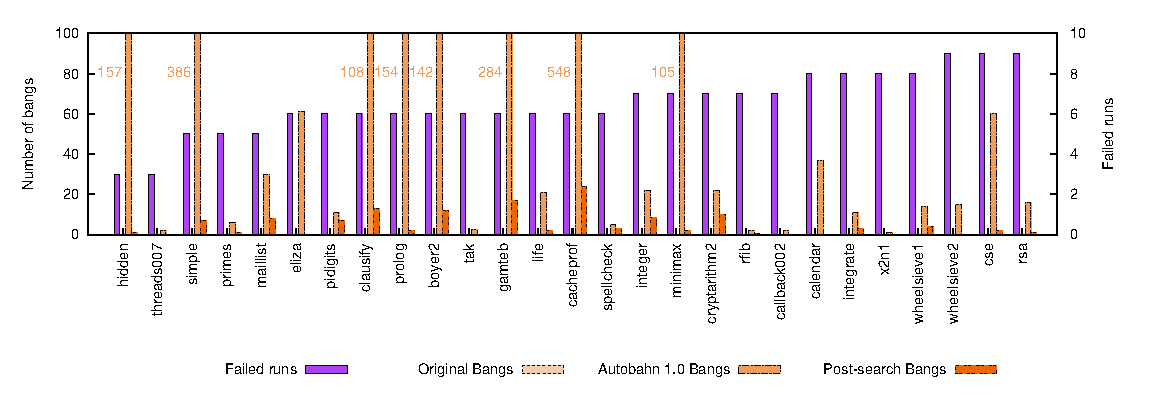
\includegraphics[width=\textwidth]{ap-partial-bangs}
\caption{Number of bangs generated by \Ao{} vs. \postopt{} phase combined with \Ao{} across 28 benchmarks. Success rate out of 10 runs is shown. Columns that exceed the maximum axis value are labelled with their actual values.}
\end{figure*}

\begin{figure*}
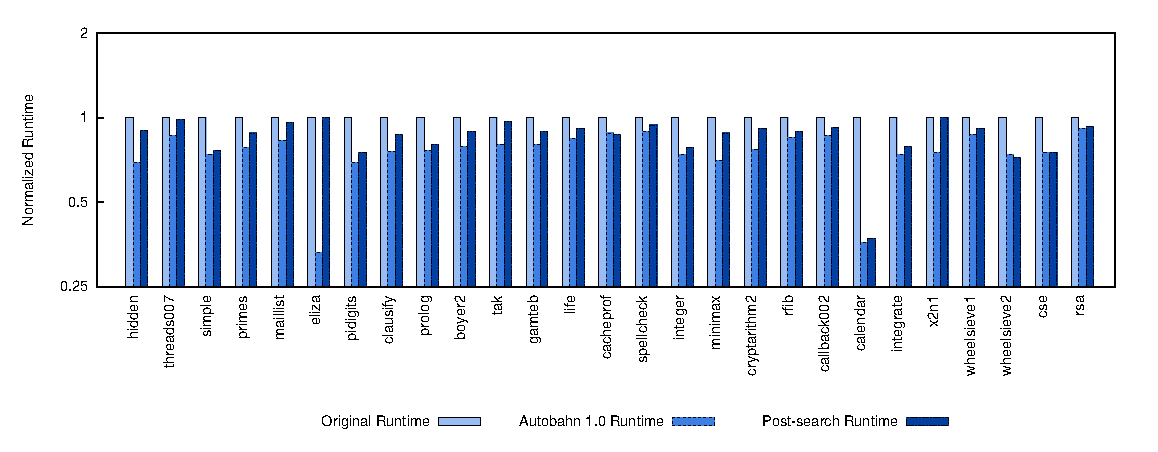
\includegraphics[width=\textwidth]{ap-partial}
\caption{Normalized runtime of \Ao{} results vs. \postopt{} phase combined with \Ao{} results across 28 benchmarks. The x-axis normalized runtime is on a log scale of base 2. Success rate out of 10 runs is shown. Columns that exceed the maximum axis value are labelled with their actual values. Benchmarks that did not terminate are indicated with a 2.0 \nonterm{} code runtime.}
\end{figure*}

\subsection{Combining \preopt{} and \postopt{}}

To test for the overall effectiveness of running \At{}, we took the average results of running both the \preopt{} and \postopt{} phase together on the 61 Autobahn benchmarks again. Out of those 61 benchmarks, 5 benchmarks were eliminated during the \preopt{} phase for having no \hotspots{} and 4 benchmarks were consistently unable to be optimized by either \At{} or \Ao{}. The remaining 52 benchmarks succeeded to optimize at least once during the ten runs, and their results are presented in figure 7, 8, 9 and 10. The benchmarks are sorted in increasing order of failure rate and split into two sets of graphs of 26 benchmarks each. Figure 7 and 9 show the results of bang reduction, and figure 8 and 10 show the corresponding runtime performances of each benchmark. 

While most benchmarks consistently showed significant bang reduction with minimally compromised performance, a few benchmarks stand out. The \texttt{expert} and \texttt{calendar} benchmark not only had bangs reduced by 79.41\% and 97.63\% respectively, but also experienced a performance speed up by 27.59\% and 14.82\% respectively. Although it is worth noting that both benchmarks failed more times than they succeeded, so such results are not guaranteed to be replicable in every run. The \texttt{atom} benchmark also has interesting results because the \postopt{} phase eliminated all bangs generated by \Ao{}, yet it still ran at 78\% of it's original runtime. This potentially suggests that \texttt{atom}'s original runtime fluctuates by a significant amount on its own. It also potentially suggests that \texttt{atom}'s overall performance improvement is achieved through the accumulation of speedups at many low-cost cost centres, so lowering \At{}'s \hotspotcost{} would help capture those cost centres with lower associated costs and result in better performance improvement.

TODO WHY PRE-aut-post HAS MORE BENCHMARKS THAN PRE-AUT

\begin{figure*}
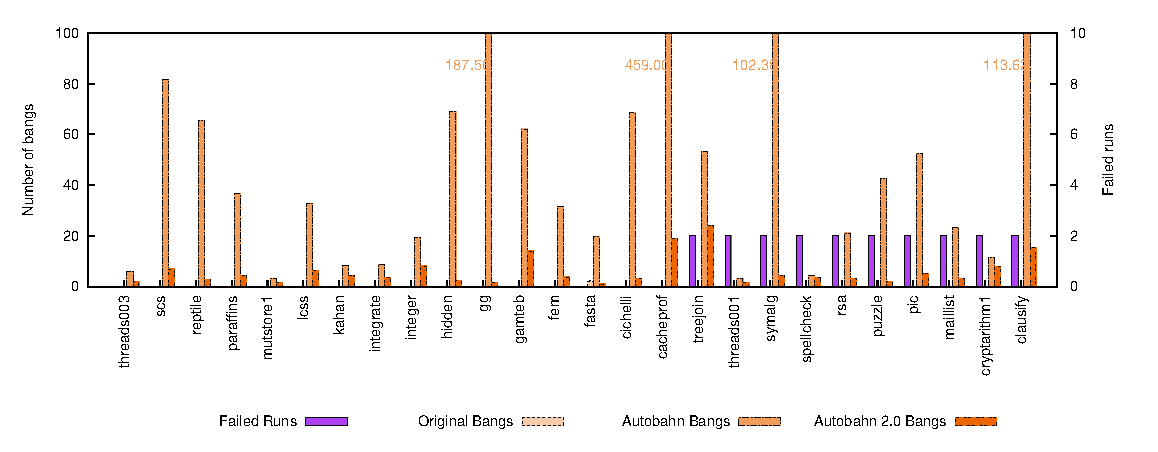
\includegraphics[width=\textwidth]{pap0-bangs}
\caption{Number of bangs generated by \Ao{} vs. \At{} across 25 benchmarks. Success rate out of 10 runs is shown. Columns that exceed the maximum axis value are labelled with their actual values.}
\end{figure*}

\begin{figure*}
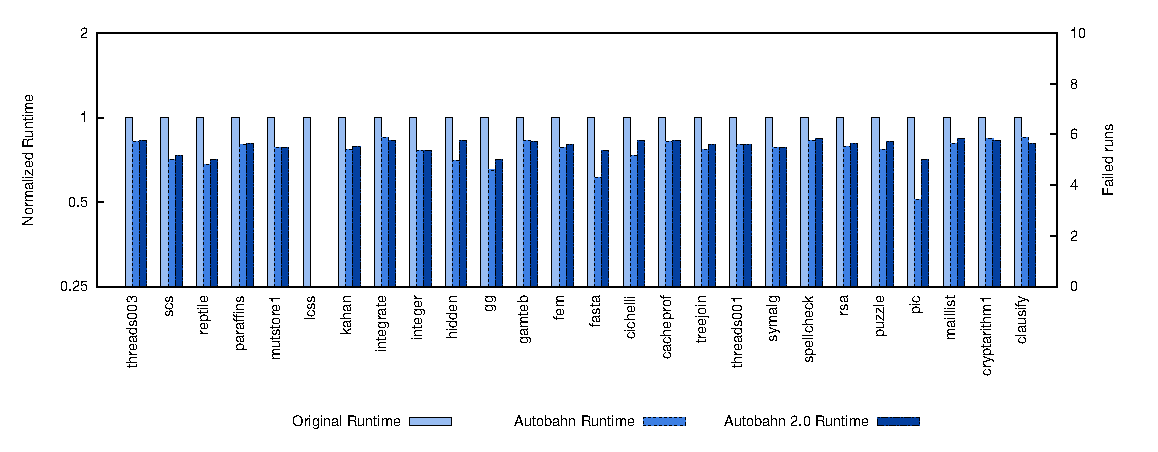
\includegraphics[width=\textwidth]{pap0}
\caption{Normalized runtime of \Ao{} results vs. \At{} results across 25 benchmarks. The x-axis normalized runtime is on a log scale of base 2. Success rate out of 10 runs is shown. Columns that exceed the maximum axis value are labelled with their actual values.}
\end{figure*}

\begin{figure*}
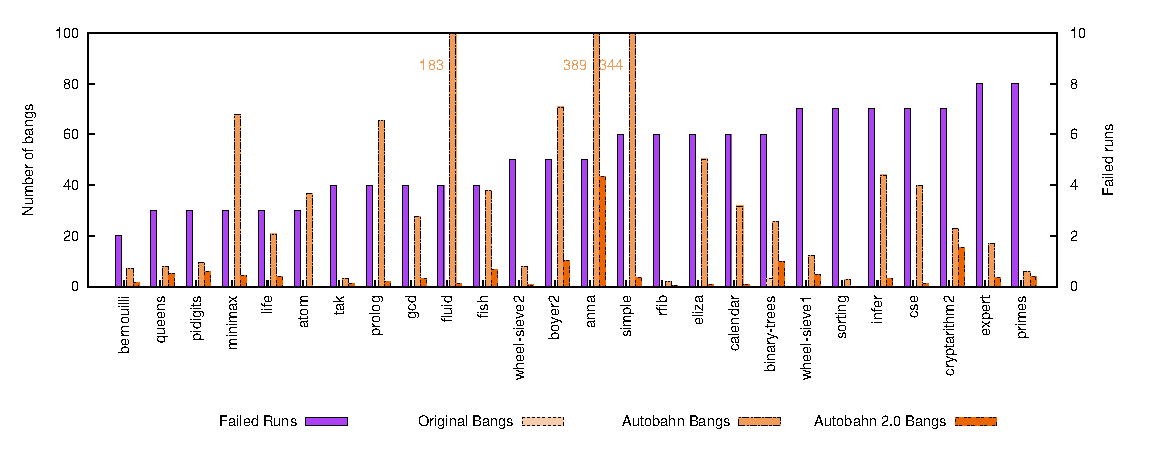
\includegraphics[width=\textwidth]{pap1-bangs}
\caption{Number of bangs generated by \Ao{} vs. \At{} across 24 benchmarks. Success rate out of 10 runs is shown. Columns that exceed the maximum axis value are labelled with their actual values.}
\end{figure*}

\begin{figure*}
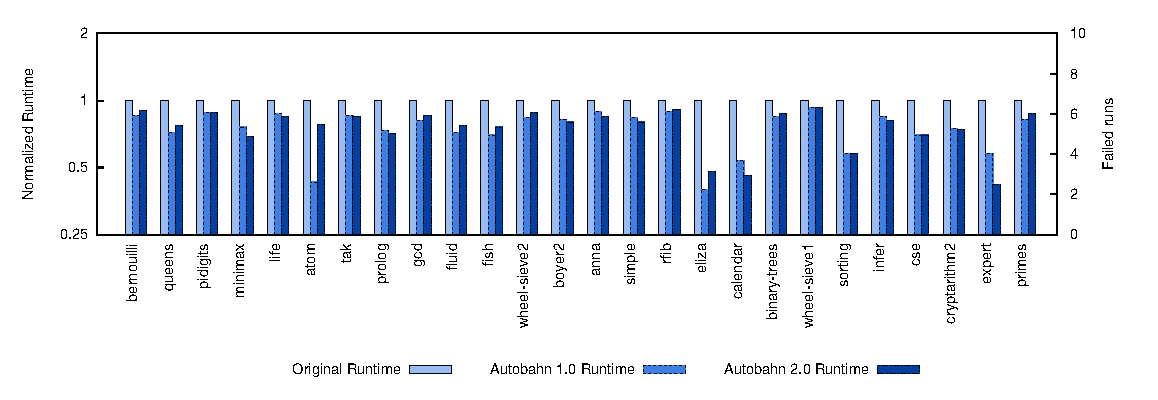
\includegraphics[width=\textwidth]{pap1}
\caption{Normalized runtime of \Ao{} results vs. \At{} results across 24 benchmarks. The x-axis normalized runtime is on a log scale of base 2. Success rate out of 10 runs is shown. Columns that exceed the maximum axis value are labelled with their actual values.}
\end{figure*}

\subsection{\At{} On Larger Programs}

We ran \At{} on the gcSimulator garbage collector to see how well it performs on larger programs. To keep optimization runtime within reasonable ranges, we used the first 1M of the batik trace file as the representative input. For gcSimulator, we lowered the \absim{} threshold to 1\% because it does not have many \hotspots{} to begin with. Once \At{} was done optimizing, we tested the resulting program on larger trace file sizes of 100M and 500M. Because running the garbage collector on the full 6184M trace size took too long with or without optimization, we did not record results for the full trace. 

The original \Ao{} was able to produce results that not only ran faster on representative input, but also on larger trace files as well. \At{} was also able to generate similar results with much fewer bangs, as demonstrated in the table below. 

\begin{tabular}{lllr}
\hline
Version   & File Size (M) & Runtime & No.Bangs \\
\hline
Original      & 1   &   0.40	 & 0   \\
          & 100        & 43.13      & 0 \\
       & 500     &  216.71 & 0 \\
\Ao{}       & 1     & 0.18    &  690\\
          & 100        & 14.19 &  690\\
                 & 500        & 68.98	& 690\\
\At{}      & 1   &  0.23 & 125    \\
          & 100        & 15.75 & 125      \\
       & 500    & 81.66 & 125    \\

\hline
\end{tabular}
 
\subsection{\At{} On Aeson}
 

 The original \Ao{} experiments also showed that its genetic algorithm was able to infer application-specific bang patterns for the \texttt{Aeson} program. The \texttt{Aeson} program is a \texttt{JSON} file parser that can be used with one of two drivers that operate differently on the \texttt{JSON} file it parses. The \texttt{validate} driver checks if the file is a valid \texttt{JSON} file without the need to completely evaluate each \texttt{JSON} value. The \texttt{convert} driver converts the \texttt{JSON} file into a Haskell data structure, and thus it needs to completely evaluate each \texttt{JSON} value. If the \texttt{Aeson} parser is paired with the \texttt{validate} driver, it performs the best when it evaluates its parsing functions lazily. If \texttt{Aeson} is paired with the \texttt{convert} driver, it performs the best when it evaluates all parsing functions eagerly. 
 
In the original \Ao{} experiment, two versions of \texttt{Aeson} were optimized. Each used one of the drivers and had the incorrect set of bangs pre-inserted to allow for room for improvement. After optimization, \Ao{} was able to correct the incorrect set of bangs by either inserting bangs in correct locations or removing bangs from incorrect locations. We were interested in seeing if \At{} preserves the same results, so we ran \At{} with identical experiment conditions to see if it preserves the correct bangs that \Ao{} produces. 

In the \preopt{} phase, \At{} identified that \texttt{Aeson}'s top hot spots were in fact located in external libraries. We followed the program's suggestions to include \texttt{Data.Attoparsec.Internal.Types} as a local file in \Ao{}'s optimization coverage. However, results showed that the inclusion of this file did not significantly improve \Ao{}'s ability to optimize \texttt{Aeson}. It is possible that external libraries and files that were suggested by the \preopt{} phase do not improve \Ao{}'s optimization runtime results, in which case it is the user's decision if they still wish to include the external files as a part of the optimization coverage. In our case, we decided to remove the newly added external file, and reran the experiment using the original setup. 


%\begin{tabular}{p{2.5cm}p{1.5cm}p{1cm}p{1.5cm}}
%\hline
%Version   & Coverage & Driver & Normalized Runtime \\
%\hline
%Original      & N/A & convert   & 1     \\
%          & N/A & validate        & 1      \\
%\Ao{}  &[\texttt{Main.hs}]      & convert     & 0.56      \\
%          &[\texttt{Main.hs}] & validate        & 0.72	\\          
%\preopt{} and \Ao{}    &  [\texttt{Main.hs}, \texttt{InternalTypes.hs}]  & convert     & 0.73     \\
 %         & [\texttt{Main.hs}, \texttt{InternalTypes.hs}]  & validate        & 0.66	\\
%\hline
%\end{tabular}


In our second run of the experiment, \Ao{} was unable to generate the correct bang patterns prior to the \preopt{} phase. Because \Ao{}'s genetic algorithm is random, every experiment will turn out slightly differently every time it is run. We were unable to use \Ao{} to reproduce the exact application-specific bang patterns for \texttt{Aeson}'s two drivers that the original paper was able to produce. Therefore, we manually inserted the correct bangs into the optimization results and resumed the bang reduction process to see if the \preopt{} phase could eliminate the useless bangs and preserve the correct bangs. We also lowered the \hotspotcost{} threshold to 0.2\% because most of the high-cost \hotspots{} were located in external libraries. 

\At{} was able to identify the key parsing function as a \hotspot{} and preserved the bang pattern in the parsing function. Therefore, the correct bang patterns produced by \Ao{} were successfully preserved in the results of \At{}. The following table illustrates the runtime and bang reduction results. 

\begin{tabular}{p{2.5cm}p{1cm}p{1.5cm}p{1.5cm}}
\hline
Version   & Driver & Normalized Runtime & No. Bangs\\
\hline
Original      & convert   & 1     & 2 \\
          & validate        & 1     &  4\\
\At{}       & convert     & 0.91     & 46\\
          & validate        & 0.86	& 93\\
\Ao{}       & convert     & 0.93     &   7 \\
          & validate        & 0.85 & 2	\\
\hline
\end{tabular}

\section{Related Work and Future Work}

\subsection{\Ao{} and Other Methods of Removing Laziness}

The current strictness analyzer in GHC uses backward abstract
interpretation to identify locations that can be eagerly
evaluated. The analysis is approximate because the analysis is
static. The analysis also conservatively binds locations as strict
only if it can guarantee program termination because it is a part of
the compiler. Autobahn has the advantage of both being dynamic and not
needing to guarantee termination on all inputs as it is not a a part
of the compiler. Instead, it allows users to decide the safety of
suggested strictness annotations based on the intended application of
the program. Other approaches to reduce laziness include Strict
Haskell~\cite{strict-haskell}, which allows users to make entire modules strict rather than
lazy by default using the -XStrict and -XStrictData language
pragmas. Chang and Felleisen starts with a program written in a strict
language, and inserts laziness annotations into it using dynamic
profiling. It would be interesting to see if Chang and Felleisen's
method could be applied to introduce laziness to Strict Haskell
programs.

\subsection{\At{} Improvements}
For future developments, it would be worth exploring the additional use of heap profiles to locate hot spots instead of solely using time and allocation profiles. We have occasionally seen programs in our experiments that may be more accurately profiled by heap usage instead of time and allocation profiles. Although it may be difficult to predict which programs' \hotspots{} are more prominently associated with heap usage, \At{} could run both profiling systems for a program and compare the profiles before selecting a more suitable one to proceed with. Another potential improvement is implementing thresholds that automatically adjust themselves based on profiling results. Our experiments show that the ideal values for \hotspotcost{} and \absim{} thresholds vary by program to program. Adopting more flexible thresholds that automatically adjust themselves after inspecting the profile in the \preopt{} phase might yield better results than using set values or asking users to provide them.


\section{Conclusion}

Laziness is a double edged sword: While it provides many benefits,
excessive laziness often causes poor performance. Strictness
annotations allow programmers to force eager evaluation, but its use
is limited to programmers with extensive experience and high levels of
expertise. Autobahn uses a genetic algorithm to automatically infer
annotations for better program performance, but it often suggests too
many bangs for users to inspect. We have built Autobahn 2.0, which
uses GHC profiling feedback to perform search space manipulation to
improve the efficiency of genetic algorithms, and eliminates bangs
based on their associated performance costs. On average, experiments
show that \At{} was able to reduce 90.9\% of generated bangs while
only compromising 3\% runtime.

\bibliographystyle{abbrvnat}
\bibliography{autobahn}

\end{document}
